\documentclass{article}

\textwidth=125mm
\textheight=200mm
\linespread{1.04}


\title{\textsc{1D Convex Regression on a Grid}}
\usepackage{marginnote}
\reversemarginpar % switch default margin to the left
\usepackage{framed}
\usepackage{xcolor}
\usepackage{nicefrac}
\usepackage{pgfplots}
\usepackage{floatrow}
\usepackage{mathtools}
\usepackage{amsthm}
\usepackage{listings}
\usepackage{tikz}
\usepackage{amssymb}
\usepackage[plain]{algorithm}
\lstset{emph={try,catch,throw,def,or,to,for,then,end,for,if,args,else,return},emphstyle=\color{blue!100!black}\textbf}
\lstset{mathescape=true,escapechar=\&,numbers=left,xleftmargin=3mm,linewidth=0.47\textwidth,framextopmargin=0pt,framexbottommargin=0pt,aboveskip=-1pt,belowskip=-1pt}
\usepackage{mdframed}
\usepackage{bm}
\usepackage[bf]{caption}
\usepackage{graphicx}
\usepackage{natbib}
\usepackage{xspace}
\usepackage[hypertexnames=false]{hyperref} % add backlinks to the end of bibliography items
\usepackage[capitalise]{cleveref}
\usepackage{autonum}

\definecolor{dkblue}{cmyk}{1,.54,.04,.19} 
\theoremstyle{plain}
\newtheorem{theorem}{Theorem}
\newtheorem{optprob}[theorem]{Optimisation Problem}
\newtheorem{lemma}[theorem]{Lemma}
\newtheorem{proposition}[theorem]{Proposition}
\newtheorem{corollary}[theorem]{Corollary}
\newtheorem{claim}[theorem]{Claim}
\theoremstyle{definition}
\newtheorem{definition}[theorem]{Definition}
\newtheorem{question}[theorem]{Question}
\newtheorem{fact}[theorem]{Fact}
\newtheorem{assumption}[theorem]{Assumption}
\newtheorem{conjecture}[theorem]{Conjecture}
\theoremstyle{plain}
\newtheorem{exampleinner}[theorem]{Example}
\newtheorem{remark}[theorem]{Remark}

% Boxed example environment with light gray background and shadow
\mdfdefinestyle{examplestyle}{%
    backgroundcolor=gray!10,
    linewidth=0.5pt,
    linecolor=gray!50,
    shadow=true,
    shadowsize=3pt,
    shadowcolor=gray!30,
    innertopmargin=8pt,
    innerbottommargin=8pt,
    innerleftmargin=10pt,
    innerrightmargin=10pt,
    skipabove=10pt,
    skipbelow=10pt
}
\newenvironment{example}[1][]{%
    \begin{mdframed}[style=examplestyle]%
    \begin{exampleinner}[#1]%
}{%
    \end{exampleinner}%
    \end{mdframed}%
}



\newcommand{\ceil}[1]{\left\lceil #1 \right\rceil}
\newcommand{\R}{\mathbb R}
\newcommand{\Rd}{\mathbb{R}^d}
\newcommand{\argmin}{\operatornamewithlimits{arg\,min}}
\newcommand{\argmax}{\operatornamewithlimits{arg\,max}}
\newcommand{\ip}[1]{\langle #1 \rangle}
\newcommand{\Reg}{\mathfrak{R}}
\newcommand{\BReg}{\mathfrak{BR}}
\newcommand{\norm}[1]{\Vert #1 \Vert}
\newcommand{\E}{\mathbb E}
\newcommand{\Z}{\mathbb Z}
\newcommand{\K}{\mathcal K}
\newcommand{\cU}{\mathcal U}
\newcommand{\cN}{\mathcal N}
\newcommand{\cT}{\mathcal T}
\newcommand{\PP}{\mathbb P}
\newcommand{\Var}{\mathbb V}
\newcommand{\cE}{\mathcal E}
\newcommand{\cK}{\mathcal K}
\newcommand{\cH}{\mathcal H}
\newcommand{\cF}{\mathcal F}
\newcommand{\cO}{\mathcal O}
\newcommand{\cS}{\mathcal S}
\newcommand{\cC}{\mathcal C}
\newcommand{\cL}{\mathcal L}
\newcommand{\cG}{\mathcal G}
\newcommand{\cA}{\mathcal A}
\newcommand{\cD}{\mathcal D}
\newcommand{\cP}{\mathcal P}
\newcommand{\BS}{\mathbb S}
\newcommand{\zeros}{ \bm 0}
\newcommand{\bbP}{\mathbb P}
\newcommand{\polylog}{\operatorname{polylog}}
\newcommand{\poly}{\operatorname{poly}}
\newcommand{\const}{\operatorname{const}}
\newcommand{\interior}{\operatorname{int}}
\newcommand{\conv}{\operatorname{conv}}
\newcommand{\diam}{\operatorname{diam}}
\renewcommand{\d}[1]{\operatorname{d}\!#1}
\newcommand{\abovelabel}[1]{\stackrel{\raisebox{0.5mm}{\textrm{\tiny \color{red} #1}}}}
\newcommand{\ta}{\tilde{a}}
\newcommand{\tP}{P'}
\newcommand{\tA}{A'}
\newcommand{\fmd}{\texttt{MD}}
\newcommand{\tfmd}{\widetilde{\texttt{MD}}}

\newcommand{\mdalg}{\textsf{MD}\xspace}
\newcommand{\smdalg}{\textsf{SMD}\xspace}
\newcommand{\expbyopt}{\textsf{ExpByOpt}\xspace}
\newcommand{\olo}{\texttt{OLO}\xspace}
\newcommand{\blo}{\texttt{BLO}\xspace}
\newcommand{\bco}{\texttt{BCO}\xspace}
\newcommand{\oco}{\texttt{OCO}\xspace}
\newcommand{\hl}{\hat{\ell}\xspace}


\begin{document}
\maketitle

Consider the $[-1, 1]$ interval and let the grid points be given by
\[
    x_i = -1 + (i-1)\Delta \qquad \text{and }\qquad \Delta = \frac{2}{d-1},
\]
for $i = 1, 2, \ldots, d$.
\begin{figure}[h]
    \centering
    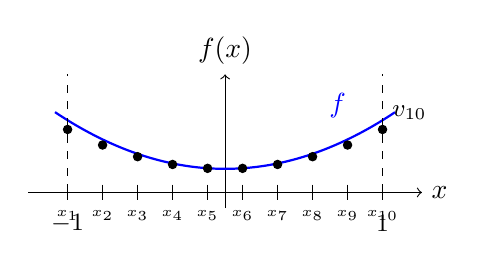
\begin{tikzpicture}
        % Axis
        \draw[->] (-2.5, 0) -- (2.5, 0) node[right] {$x$};
        \draw[->] (0, -0.2) -- (0, 1.5) node[above] {$f(x)$};

        % The Convex Function Curve (f(x) = 0.5x^2 + 0.3)
        \draw[thick, blue, domain=-1.2:1.2, samples=100] plot (\x*1.8, {0.5*(\x)^2 + 0.3});
        \node[blue, right] at (1.2, 1.1) {$f$};

        % Grid points and vertical projection to the function
        \foreach \i in {1, ..., 10} {
                % Calculate x coordinate from -1 to 1 based on your formula
                \pgfmathsetmacro{\xval}{-1 + (\i-1)*2/9}
                % Scale for visualization (multiplying by 2 to stretch across the TikZ canvas)
                \pgfmathsetmacro{\xplot}{\xval * 2}
                \pgfmathsetmacro{\yplot}{0.5*(\xval)^2 + 0.3}

                % Draw tick marks on x-axis
                \draw (\xplot, 0.1) -- (\xplot, -0.1) node[below] {\tiny $x_{\i}$};

                % Draw points v_i = f(x_i)
                \filldraw[black] (\xplot, \yplot) circle (1.5pt);
                \ifnum\i=10
                    \node[above right] at (\xplot, \yplot) {\small $v_{10}$};
                \fi
            }

        % Label the interval boundaries
        \draw[dashed] (-2, 0) -- (-2, 1.5);
        \draw[dashed] (2, 0) -- (2, 1.5);
        \node at (-2, -0.4) {\small $-1$};
        \node at (2, -0.4) {\small $1$};

    \end{tikzpicture}
    \caption{A sample convex function $f$ and the resulting convex vector $\bm{v}$ where $v_i = f(x_i)$ on the grid $d=10$.}
    \label{fig:grid_points}
\end{figure}

A \emph{convex vector} on this grid is a vector $v \in \R^{d}$ such that there exists a \textbf{bounded} convex function $f: [-1, 1] \to [0, 1]$ satisfying $v_i = f(x_i)$ for all $i = 1, \ldots, d$. The set of all convex vectors on this grid is denoted by $\cC_d$.

Let $E:[d] \times [0, 1] \to \Rd$ be an \emph{estimation function} that maps each index $i \in [d]$ and value $v_i \in [0, 1]$ to a vector in $\Rd$.
Our goal can roughly be stated as follows:
find an estimation function $E$ such that given a convex vector $v \in \cC_d$, and a distribution $p \in \Delta(d)$, we have
\begin{align}
    v \approx \sum_{i=1}^d p_i E(i, v_i)\,,
\end{align}
while $\|E(i, v_i)\|$ is not too large for each $i \in [d]$.

\section{The objective}
Before stating our objective, we introduce some notation.
Let $q \in \Delta(d)$ be an arbitrary distribution (prior)
and $p \in \Delta(d)$ be another distribution (policy) that we optimize over.
Let
\begin{align}
    \bar{v} = \sum_{j=1}^d p_j E(j, v_j)\,.
\end{align}
We measure the quality of the estimation function $E$ and a policy $p$ using the following two quantities:
\begin{enumerate}
    \item The bias term:
          \begin{align}
              \Lambda_{\text{bias}, q}(E, p ; v) :=
              \langle p, v\rangle - \langle q, \bar{v} \rangle
              +
              \max_{i \in [d]} \langle e_i, \bar{v}- v \rangle\,.
          \end{align}
    \item The variance term:
          \begin{align}
              \Lambda_{\text{var}, q}(E, p ; v) :=
              %   D_{F^\star}(F'(q) - \eta E(j, v_j), F'(q))
              %   \abovelabel{(a)}
              %   \leq
              \sum_{i=1}^d \sum_{j=1}^d q_i p_j E(j, v_j)_i^2\,,
          \end{align}
          %   where $F$ the unnormalized negative Shannon entropy defined as $F(x) = \sum_{i=1}^d x_i \log x_i$ for $x \in \R_+^d$, and $D_{F^\star}$ is the Bregman divergence associated with the Fenchel conjugate of $F$.
          %   We prove the inequality in (a) later.
\end{enumerate}

Our goal is to find an estimation function $E:[d] \times [0, 1] \to \Rd$, and a policy $p \in \Delta(d)$ such that
\begin{align}
    \Lambda_q(E, p ; v) := d \cdot \Lambda_{\text{bias}, q}(E, p ; v) + \Lambda_{\text{var}, q}(E, p ; v)\,,
\end{align}
is minimized for the worst case convex vector $v \in \cC_d$.

\subsection{The value of $\Lambda$ for the trivial estimation function.}
A simple choice of the estimation function is
\begin{align}
    E(i, v_i) = p_i^{-1} \cdot v_i \cdot e_i\,,
\end{align}
where $e_i$ is the $i$-th standard basis vector in $\R^d$.
This gives
\begin{align}
    \sum_{i=1}^d p_i E(i, v_i) = \sum_{i=1}^d p_i \cdot p_i^{-1} \cdot v_i \cdot e_i = \sum_{i=1}^d v_i \cdot e_i = v\,.
\end{align}
This choice perfectly reconstructs the vector $v$ and is also not limited to convex vectors.
The problem with this estimator is that the variance of the estimation vectors $E(i, v_i)$ can be very large,
i.e., $\|E(i, v_i)\|$ can be as large as $d$ for each $i \in [d]$. We will elaborate on this point later.
For the trivial estimation function defined earlier, we have $\bar{v} = v$.
Therefore, by choosing $p =q$, we have
\begin{align}
    \Lambda_{\text{bias}, q}(E, q ; v)
    = \langle q, v\rangle - \langle q, v \rangle
    + \max_{i \in [d]} \langle e_i, v - v \rangle
    = 0 + 0 = 0\,.
\end{align}
Thus, the bias term is zero.
For the variance term, we have
\begin{align}
    \Lambda_{\text{var}, q}(E, q ; v)
    =
    \sum_{i=1}^d \sum_{j=1}^d q_i p_j E(j, v_j)_i^2
    = \sum_{i=1}^d \sum_{j=1}^d q_i q_j \left( q_j^{-1} v_j \mathbf{I}\{i= j\} \right)^2
    = \sum_{j=1}^d v_j^2 \leq d\,,
\end{align}
since $v_i \in [0, 1]$ for all $i \in [d]$.
Therefore, for the trivial estimation function, we already have an upper bound of $d$ on the value of interest $\Lambda_q(E, p ; v)$ for any convex vector $v \in \cC_d$.
Note that \textbf{we didn't use the convexity of $v$} in this calculation and this upper bound holds for any vector $v \in [0, 1]^d$.

\subsection{The extreme points of $\cC_d$.}
The material in this section is not used in the rest of analysis, but it is interesting in its own right and may be useful to make progress.
\begin{theorem}
    The set $\cC_d$ can be characterized as convex hall of the vectors $u_{a,b} \in \R^d$ defined for $1\leq a \leq b \leq d$ as
    \[
        (u_{a,b})_i = \begin{cases}
            1 - \frac{x_i + 1}{x_a + 1} & \text{if } i \leq a,  \\
            0                           & \text{if } a < i < b, \\
            \frac{x_i - b}{1 - x_b}     & \text{if } b \leq i.
        \end{cases}
    \]
    Moreover, this is the unique minimal set with such a property.
\end{theorem}

\begin{figure}[h]
    \centering
    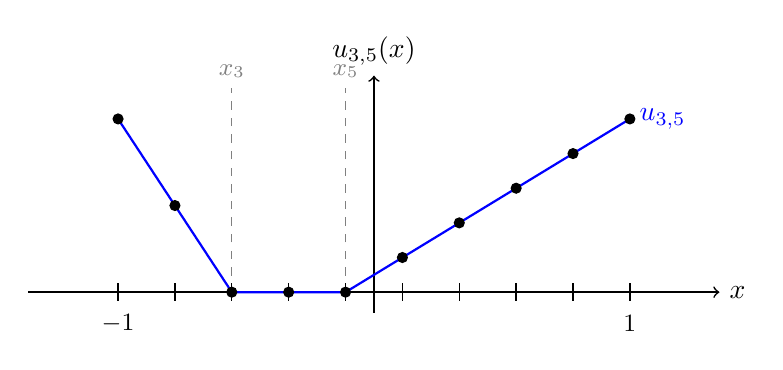
\begin{tikzpicture}[x=3.25cm,y=2.2cm] % <-- bigger overall (both axes)
        % parameters
        \pgfmathsetmacro{\d}{10}
        \pgfmathsetmacro{\a}{3}
        \pgfmathsetmacro{\b}{5}
        \pgfmathsetmacro{\xa}{-1 + 2*(\a-1)/(\d-1)}
        \pgfmathsetmacro{\xb}{-1 + 2*(\b-1)/(\d-1)}

        % axes
        \draw[->, line width=0.6pt] (-1.35, 0) -- (1.35, 0) node[right] {$x$};
        \draw[->, line width=0.6pt] (0, -0.12) -- (0, 1.25) node[above] {$u_{3,5}(x)$};

        % piecewise-linear shape of u_{3,5}
        \draw[thick, blue]
        (-1,1) -- (\xa,0) -- (\xb,0) -- (1,1);
        \node[blue, right] at (1,1) {$u_{3,5}$};

        % mark a and b breakpoints
        \draw[dashed, gray] (\xa,0) -- (\xa,1.18);
        \draw[dashed, gray] (\xb,0) -- (\xb,1.18);
        \node[gray, above] at (\xa,1.18) {\small $x_3$};
        \node[gray, above] at (\xb,1.18) {\small $x_5$};

        % grid points, ticks, and values
        \foreach \i in {1,...,10} {
                \pgfmathsetmacro{\xi}{-1 + 2*(\i-1)/(\d-1)}

                \pgfmathparse{(\i<=\a) ? (1 - (\xi+1)/(\xa+1)) : ((\i<\b) ? 0 : ((\xi-\xb)/(1-\xb)))}
                \let\yi\pgfmathresult

                \draw[line width=0.5pt] (\xi, 0.05) -- (\xi, -0.05);
                \filldraw[black] (\xi, \yi) circle (1.8pt);
            }

        % interval endpoints
        \node at (-1, -0.18) {\small $-1$};
        \node at (1, -0.18) {\small $1$};
    \end{tikzpicture}
    \caption{Example \(u_{3,5}\) on the grid \(d=10\).}
\end{figure}

The significance of this characterization is that to evaluate the worst-case performance of an estimation function $E$ and a policy $p$, it suffices to consider only the extreme points $u_{a,b}$ of $\cC_d$ instead of all convex vectors in $\cC_d$.
This is because the objective function $\Lambda_q(E, p ; v)$ is convex in $v$, and the maximum of a convex function over a convex set is attained at an extreme point of that set.

\section{Affine estimators}
To make the problem more tractable, we further restrict the search space of estimation functions.
Specifically, we only consider estimation functions of the form
\begin{align}
    E(i, v_i) = v_i \cdot s_i + b_i\,,
\end{align}
where $s_i, b_i \in \R^d$ for each index $i \in [d]$.
With this form, a function $E$ is fully specified by the two matrices $S = [s_1, s_2, \ldots, s_d]$ and $B = [b_1, b_2, \ldots, b_d]$ in $\R^{d \times d}$.
So our design problem is
\begin{align}
    \inf_{S, B \in \R^{d \times d}, p \in \Delta(d)} \sup_{v \in \cC_d} \Lambda(E_{S,B},p; v)
    = \inf_{S, B \in \R^{d \times d}, p \in \Delta(d)} \sup_{(a,b)} \Lambda(E_{S,B},p; u_{a,b})\,,
\end{align}
where $E_{S,B}$ is the estimation function defined by matrices $S$ and $B$,
and the last equality follows from the convexity of $\Lambda$ in $v$ and the fact that $\cC_d$ is the convex hull of the extreme points $u_{a,b}$.

The following lemma is not used in the rest of the analysis, but it is interesting in its own right and may be useful to make progress.
\begin{lemma}[Column-wise $q$--centering helps]
    \label{lem:q_centering}
    Fix $q\in\Delta(d)$. For any $(S,B,p)$, define centered columns
    \begin{align}
        s_j' := s_j - \langle q,s_j\rangle\,\mathbf{1},
        \qquad
        b_j' := b_j - \langle q,b_j\rangle\,\mathbf{1},
        \qquad \forall j\in[d],
    \end{align}
    and let $S',B'$ be the matrices with columns $(s_j')_{j=1}^d,(b_j')_{j=1}^d$.
    Then for every $v\in[0,1]^d$ and every $p\in\Delta(d)$,
    \begin{align}
        \Lambda_{\text{bias},q}(E_{S',B'},p;v) = \Lambda_{\text{bias},q}(E_{S,B},p;v),
        \qquad
        \Lambda_{\text{var},q}(E_{S',B'},p;v) \le \Lambda_{\text{var},q}(E_{S,B},p;v).
    \end{align}
    Consequently, there exists an optimal solution to
    $\inf_{S,B,p}\sup_{v\in\cC_d}\Lambda_q(E_{S,B},p;v)$ satisfying
    $\langle q,s_j\rangle=\langle q,b_j\rangle=0$ for all $j$.
\end{lemma}
\noindent The proof is deferred to \ref{proof:lem:q_centering}.

\subsection{Convex formulation of the design problem.}
\label{sec:convex_program_formulation}
With further work, this problem can be cast as a convex optimization problem.
We can formulate this problem as a QCQP as
\[
    \boxed{
        \begin{array}{ll}
            \text{minimize}_{S,B,t,\theta_{a,b}} & t                                                                                                 \\[1mm]
            \text{subject to}
                                                 & \theta_{a,b} \ge \frac{1}{d} \langle \mathbf{1} - d e_k, (d I - S) u_{a,b} - B \mathbf{1} \rangle
            \quad \forall 1\le a\le b\le d,\ \forall k\in[d],                                                                                        \\[1mm]
                                                 & t \ge \theta_{a,b}+\frac{1}{d^2}\sum_{i=1}^d\|(u_{a,b})_i s_i+b_i\|^2
            \quad \forall 1\le a\le b\le d\,,
        \end{array}
    }
\]
for $p = q = \frac{1}{d} \mathbf{1}$.
And in general for any $p, q \in \Delta(d)$, we have the following for a fixed prior policy $q$ and exploration policy $p$:
\[
    \boxed{
        \begin{array}{ll}
            \text{minimize}_{S,B,t,\theta_{a,b}} & t                                                                                                                                           \\[1mm]
            \text{subject to}
                                                 & \theta_{a,b} \ge \frac{1}{d}\left(\langle p - e_k, u_{a,b} \rangle - \langle q - e_k, (S \operatorname{diag}(u_{a,b}) + B) p \rangle\right)
            \quad \forall 1\le a\le b\le d,\ \forall k\in[d],                                                                                                                                  \\[1mm]
                                                 & t \ge \theta_{a,b}+\sum_{i=1}^d \sum_{j=1}^d q_i p_j ((u_{a,b})_j s_{i,j} + b_{i,j})^2
            \quad \forall 1\le a\le b\le d\,,
        \end{array}
    }
\]
using which we can further optimize over $p \in \Delta(d)$ to get the final solution.

\subsection{Exponential kernel estimators}
Numerical optimization on the formulated problem in \cref{sec:convex_program_formulation}
suggests that a good solutions $(S,B,p)$ to the optimization problem exhibit the following shape
\begin{align}
    s_{i,j} \approx A_i B_j \cdot \exp(-\lambda_i |i-j|),
    \qquad
    b_{i,j} \approx - C_i D_j \cdot \exp(-\mu_i |i-j|),
\end{align}
for some constants $A_i, B_j, C_i, D_j, \lambda_i,\mu_i>0$ depending on the column index $i$ and row index $j$.
We call such estimators \emph{exponential estimators}, and explore their properties now.
But First we introduce the continuous setting to explain a formulation of the problem.

\subsection{The continuous problem}
We switch to the continuous setting on $[-1,1]$ to explain the observed structure.
Formally, imagine that instead of an index $i\in[d]$ we observe a location $x\in[-1,1]$, sample $x\sim p$, and observe $f(x)\in[0,1]$ for an unknown convex function $f$.
An affine estimator in this setting is a map
\begin{align}
    E: [-1,1]\times[0,1]\to L^\infty([-1,1]),\qquad
    E(x,f(x))(\,\cdot\,)= f(x)\,s_x(\,\cdot\,) + b_x(\,\cdot\,),
\end{align}
and the average estimate is
\begin{equation}
    \bar f(t) := \int_{-1}^1 p(x)\,E(x,f(x))(t)\,dx
    = \int_{-1}^1 p(x)\,\bigl(f(x)s_x(t)+b_x(t)\bigr)\,dx.
    \label{eq:barf_def}
\end{equation}

\paragraph{The probabilistic view}
The overall goal is to design $S, B$ and $p$ jointly to minimize the worst-case value of $\Lambda_q$.
In this section we basically re-parametrize this joint design problem in a way that makes the structure of the solution more transparent.

Fix some $p$.
Define
\begin{align}
    Z(t) := \int_{-1}^{1} p(x) s_x(t) \,dx\,.
\end{align}
Suppose that $p(x)$ and $s_x(t)$ are such that $Z(t) \neq 0$ for all $t$ (which is the case for exponential kernels).
Then, we can define a new function $h(x|t)$ as
\begin{align}
    h(x|t) := \frac{p(x) s_x(t)}{Z(t)}\,, \qquad \text{so that} \qquad \int_{-1}^{1} h(x|t) \, dx = 1.
\end{align}

The idea is that \textbf{if we restrict to nonnegative kernels $s_x(t) \ge 0$},
then instead of designing $s_x(t)$ directly, we can equivalently design $h(\cdot|t)$ on $[-1,1]$ for each $t$,
and the scaling factors $Z_t$ for each $t$.

Starting from the continuous form $\bar{f}$ , we have
\begin{align}
    \bar{f}(t) & = \int_{-1}^{1} p(x) s_x(t) f(x) \,dx + \underbrace{\int_{-1}^{1} p(x)\,b_x(t)}_{:=C(t)}\,dx \\
               & = Z(t) \cdot \int_{-1}^{1} h(x|t) f(x) \, dx + C(t)                                          \\
               & = Z(t) \cdot \E_{x\sim h(\cdot|t)}[f(x)] + C(t)\,.
\end{align}
The take away message is that, when we restrict to nonnegative kernels, the design of the estimator can be viewed as the design
of a family of (kernel) distributions $h(\cdot|t)$ on $[-1,1]$ for each $t$, and the scaling and bias factors $Z(t)$ and $C(t)$ for each $t$.

\subsection{A $\sqrt{d \log(d)}$ upper bound on \texorpdfstring{$\Lambda$}{Lambda}}
\label{sec:kernel_exp_family_bound}
In this section we show that by designing the kernel distributions $h(\cdot|t)$ to be concentrated around $t$, we can get a much better upper bound on $\Lambda$ than the trivial estimator.
Motivated by the probabilistic view in the previous section, we restrict to estimators of the form
\begin{align}
    \label{eq:S_from_pi}
    s_j(t) = \frac{z(t) \cdot h(j|t)}{p_j},
\end{align}
where $h(j|t)$ is a distribution on $[d]$ for each $t$.
Equivalently, the estimator outputs the vector
\begin{align}
    E_{h}(j,v_j)_t := v_j \cdot \frac{z_t \cdot h(j|t)}{p_j}.
\end{align}
Note that the our estimator particularly has zero intercept term ($B\equiv 0$), i.e., $b_j=0$ for all $j$, and $z_t = 1$ for all $t$.

For any $v\in\R^d$ and any $t\in[d]$, the average estimate at location $t$ is
\begin{align}
    \bar v_t := \sum_{j=1}^d p_j E_{h}(j,v_j)_t
    = z_t \sum_{j=1}^d h(j|t) v_j
    = z_t \cdot \E_{J\sim h(\cdot|t)}[v_J]\,.
\end{align}

\subsubsection{Local Lipschitz bounds for convex functions}
Whatever we did so far is valid for any vector $v\in[0,1]^d$.
We now bound the pointwise error $\bar v_i-v_i$ for convex vectors $v\in\cC_d$.
\begin{lemma}[A one-sided Lipschitz bound for bounded convex functions]
    \label{lem:convex_one_sided_lip}
    Let $f:[-1,1]\to[0,1]$ be convex. Then for any $t\in(-1,1)$ and any $x\in[-1,1]$,
    \begin{equation}
        f(x)-f(t) \le \frac{|x-t|}{1-|t|}.
        \label{eq:convex_one_sided_lip}
    \end{equation}
\end{lemma}
\noindent The proof is deferred to \ref{proof:lem:convex_one_sided_lip}.

\begin{proposition}[Bias bound via the first absolute moment]
    \label{prop:bias_first_moment}
    Consider the kernel estimator $E_h$ defined above, then for each $t$ we have
    \begin{equation}
        \bar v_t - v_t
        \le \frac{1}{1-|x_t|}\E_{J\sim h(\cdot|t)}\left[|x_J-x_t|\right]\,.
        \label{eq:pointwise_bias_bound}
    \end{equation}
\end{proposition}
\noindent The proof is deferred to \ref{proof:prop:bias_first_moment}.

\eqref{eq:pointwise_bias_bound} can be seen as a local Lipschitz bound for convex functions, where the local Lipschitz constant at $t$ is $\frac{1}{1-|x_t|}$.
The significance is that by designing the kernel $h(\cdot|t)$ concentrated around $t$, we can control the bias term $\bar v_t-v_t$ for convex vectors $v$.

\begin{remark}
    Assume the \emph{barycenter condition}
    \begin{equation}
        \E_{J\sim h(\cdot|t)}[x_J] = x_t,\qquad \forall t\in[d]\,;
        \label{eq:barycenter_condition}
    \end{equation}
    then
    \begin{align}
        0 \le \bar v_t - v_t\,,
    \end{align}
    by Jensen's inequality, and in particular, when $p=q$,
    \begin{equation}
        \Lambda_{\mathrm{bias},q}(E_h,p;v)
        = \langle q,v\rangle-\langle q,\bar v\rangle + \max_{t\in[d]}(\bar v_t-v_t)
        \le \max_{t\in[d]}(\bar v_t-v_t).
        \label{eq:Lambda_bias_bound_by_max}
    \end{equation}
\end{remark}

\subsubsection{Laplace kernel and kernel policies}
The goal here is to extend the above analysis to the case where $q$ is an arbitrary distribution on $[d]$.
\paragraph{The choice of $p$.}
The first question is how to choose $p$.
A compelling choice is
\begin{align}
    p_j = \sum_{t=1}^{d} q_t h(j|t)\,,
\end{align}
which is a valid probability distribution.
We call this choice the \emph{kernel policy} associated with the kernel $h$.
Then
\begin{align}
    \langle q, \bar v\rangle & = \sum_{t=1}^d q_t \bar v_t
    = \sum_{t=1}^d q_t z_t \cdot \left(\sum_{j=1}^d h(j|t) v_j\right)
    = \sum_{j=1}^d v_j \sum_{t=1}^d q_t h(j|t) \cdot z_t
    = \sum_{j=1}^d v_j p_j
    = \langle p, v\rangle\,,
\end{align}
which gives
\begin{align}
    \Lambda_{\mathrm{bias},q}(E_h,p;v)
     & = \langle p ,v\rangle-\langle q,\bar v\rangle + \max_{t\in[d]}(\bar v_t-v_t)
    = \max_{t\in[d]}(\bar v_t-v_t)\,,
\end{align}
which holds regardless of what $q$ is.
\paragraph{The choice of $h$}
We define
\begin{align}
    h(j|t) \propto e^{-\lambda_t |j-t|}\,,
\end{align}
where $\lambda_t$ is a parameter depending on $t$ that controls the concentration of the kernel around $t$.
Precisely, $h(\cdot|t) = \cL(\lambda_t, t)_{[d]}$ is the truncated Laplace distribution on $[d]$ with center $t$ and parameter $\lambda_t$.

\paragraph{Bounding the value of $\Lambda_{\textrm{bias}}$}
With the local Lipschitz bound from Proposition~\ref{prop:bias_first_moment}
and the choice of $p$ and $h$, we can bound the bias term as
\begin{align}
    \Lambda_{\mathrm{bias}, q}(E_h, p ; v)
    \le \max_{t\in[d]}\frac{\E_{J\sim h(\cdot|t)}\left[|x_J-x_t|\right]}{1-|x_t|}
    = \max_{t\in[d]}\frac{\Delta}{1-|x_t|}\E_{J\sim h(\cdot|t)}\left[|J-t|\right]\,,
\end{align}
where we have $J \sim \cL(\lambda_t, t)_{[d]}$.
Therefore, we need a bound on the first absolute moment of the truncated Laplace distribution $\cL(\lambda, t)_{[d]}$,
in terms of the parameter $\lambda_t$.
It's not hard to prove that the truncation only decreases the first absolute moment for a symmetric distribution, so we can use the first absolute moment of the untruncated Laplace distribution, which is $\frac{1}{\sinh(\lambda_t)}$ provided by the next lemma.
\begin{lemma}[Moments of the symmetric discrete Laplace law on $\Z$]
    \label{lem:discrete_laplace_moments}
    Let $K$ have the symmetric discrete Laplace law:
    $\PP(K=k) = \frac{1-\rho}{1+\rho} \cdot \rho^{|k|}$ for $k\in\Z$ and $\rho = e^{-\lambda}$ for some $\lambda > 0$.
    Then
    \begin{equation}
        \E\left[|K|\right] = \frac{1}{\sinh(\lambda)} \le \frac{1}{\lambda}.
        \label{eq:laplace_abs_moment}
    \end{equation}
\end{lemma}
\noindent The proof is deferred to \ref{proof:lem:discrete_laplace_moments}.

Therefore, let $\alpha \ge 1$ be a parameter,
by setting $\lambda_t = \alpha\Delta/(1-|x_t|)$, we get
\begin{align}
    \Lambda_{\mathrm{bias}, q}(E_h, p ; v)
    \le \max_{t\in[d]}\frac{\Delta}{1-|x_t|}\cdot \frac{1}{\sinh(\lambda_t)}
    \le \max_{t\in[d]}\frac{\Delta}{1-|x_t|}\cdot \frac{1}{\lambda_t}
    = \frac{1}{\alpha}\,.
\end{align}

\paragraph{The bound on $\Lambda_{\mathrm{var}}$}
For the variance term, we have
\begin{align}
    \Lambda_{\text{var}, q}(E_h, p ; v)
     & =
    \sum_{t=1}^d \sum_{j=1}^d q_t p_j E_h(j, v_j)_t^2
    = \sum_{t=1}^d \sum_{j=1}^d q_t p_j \left(v_j \cdot \frac{z_t \cdot h(j|t)}{p_j}\right)^2 \\
     & = \sum_{t=1}^d \sum_{j=1}^d q_t \frac{v_j^2 z_t^2 h(j|t)^2}{p_j}
    \abovelabel{(a)}{\leq} \sum_{t=1}^d \sum_{j=1}^d q_t \frac{ h(j|t)^2}{p_j}\,,
\end{align}
where (a) holds since $v_j\in[0,1]$.
Since we use the discrete Laplace kernel $h(j|t) \propto e^{-\lambda_t |j-t|}$, we have $h(j|t) \leq h(j|j)$ for all $t$.
Therefore, we can write
\begin{align}
    \Lambda_{\text{var}, q}(E_h, p; v)
     & \le \sum_{j=1}^d \frac{h(j|j)}{p_j}\sum_{t=1}^d q_t h(j|t)
    \abovelabel{(a)}{=} \sum_{j=1}^d h(j|j)\,,
\end{align}
where we have used the definition of $p_j$ in (a).
Next, we need an upper bound on $h(j|j)$, where $h(\cdot|j)$ is the truncated Laplace distribution on $[d]$ with center $j$ and parameter $\lambda_j$, which is given by the next lemma.
\begin{lemma}
    \label{lem:truncated_laplace_mass_at_center}
    Let $X \sim \cL(\lambda, j)_{[d]}$ be the truncated Laplace distribution on $[d]$ with center $j$ and parameter $\lambda$, then
    \begin{align}
        \mathbb{P}(X=j) \le \frac{1-e^{-\lambda}}{1-e^{-\lambda d}}\,.
    \end{align}
\end{lemma}
\noindent The proof is deferred to \ref{proof:lem:truncated_laplace_mass_at_center}.

Recall that $x_t = -1 + (t-1)\Delta$ and $\Delta = \frac{2}{d-1}$,
and observe that the choice $\lambda_t=\alpha\Delta/(1-|x_t|)$ from the previous subsection is equivalently
\begin{equation}
    \lambda_t=\frac{\alpha}{\min\{t-1,\ d-t\}}
    \qquad (t=2,\ldots,d-1),
    \label{eq:lambda_by_distance_to_boundary}
\end{equation}
and we interpret $\lambda_1=\lambda_d=+\infty$, i.e.\ $h(\cdot|1)=\delta_1$ and $h(\cdot|d)=\delta_d$.

Continuing from the variance bound, and using Lemma~\ref{lem:truncated_laplace_mass_at_center}, we have
\[
    \Lambda_{\text{var}, q}(E_h, p; v)\le \sum_{j=1}^d h(j|j)
    \leq 2 + \sum_{j=2}^{d-1} \frac{1 - e^{-\lambda_j}}{1 - e^{-\lambda_j d}}\,,
\]
Under the parametrization \eqref{eq:lambda_by_distance_to_boundary}, for $j\in\{2,\ldots,d-1\}$ we have
$\min\{j-1,d-j\}\le \frac{d-1}{2}$, hence
\begin{equation}
    \lambda_j d
    = \frac{\alpha d}{\min\{j-1,d-j\}}
    \ge \frac{\alpha d}{(d-1)/2}
    \ge 2\alpha.
    \label{eq:lambda_d_lowerbound}
\end{equation}
Therefore $1-e^{-\lambda_j d}\ge 1-e^{-2\alpha}$, and for $\alpha\ge 1$ we also have
$1-e^{-2\alpha}\ge 1-e^{-2}$.
Combining these with $1-e^{-u}\le \min\{1,u\}$ yields the uniform bound
\begin{equation}
    h(j|j)
    \le \frac{1}{1-e^{-2}}\,(1-e^{-\lambda_j})
    \le \frac{1}{1-e^{-2}}\,\min\{1,\lambda_j\},
    \qquad j=2,\ldots,d-1.
    \label{eq:center_mass_bound_simple}
\end{equation}
For the endpoints, $h(1|1)=h(d|d)=1$ by definition.

It remains to upper bound the sum $\sum_{j=2}^{d-1}\min\{1,\lambda_j\}$ with $\lambda_j$ as in \eqref{eq:lambda_by_distance_to_boundary}.

\begin{lemma}[A harmonic bound for the Laplace widths]
    \label{lem:harmonic_sum_lambda}
    Fix $\alpha\ge 1$ and $d\ge 3$, and define $\lambda_j=\alpha/\min\{j-1,d-j\}$ for $j=2,\ldots,d-1$.
    Then
    \begin{equation}
        \sum_{j=2}^{d-1}\min\{1,\lambda_j\}
        \le 2\alpha\bigl(1+\log d\bigr).
        \label{eq:harmonic_sum_lambda}
    \end{equation}
\end{lemma}
\noindent The proof is deferred to \ref{proof:lem:harmonic_sum_lambda}.

\begin{proposition}[A $\sqrt{d\log d}$ guarantee for general $q$ (with $z\equiv 1$ and $B\equiv 0$)]
    \label{prop:sqrt_dlogd_general_q}
    Fix an arbitrary prior $q\in\Delta(d)$.
    Let $\alpha\ge 1$ and define kernels $h(\cdot|t)$ on $[d]$ as truncated Laplace distributions centered at $t$
    with parameter $\lambda_t$ given by \eqref{eq:lambda_by_distance_to_boundary} for $t=2,\ldots,d-1$,
    and $h(\cdot|1)=\delta_1$, $h(\cdot|d)=\delta_d$.
    Define the exploration policy
    \begin{equation}
        p_j := \sum_{t=1}^d q_t\,h(j|t),\qquad j\in[d],
        \label{eq:p_as_q_mixture}
    \end{equation}
    and the (nonnegative-kernel) affine estimator with $z_t\equiv 1$ and $b\equiv 0$:
    \[
        E_h(j,v_j)_t := v_j\cdot \frac{h(j|t)}{p_j}.
    \]
    Then for every convex vector $v\in\cC_d$,
    \begin{align}
        \label{eq:Lambda_bound_general_q}
        \Lambda_q(E_h,p;v)
        \le
        \frac{d}{\alpha}
        + \frac{1}{1-e^{-2}}\Bigl(2 + 2\alpha(1+\log d)\Bigr).
    \end{align}
    In particular,
    \[
        \sup_{v\in\cC_d}\Lambda_q(E_h,p;v)
        = O\!\left(\sqrt{d\log d}\right),
    \]
    by taking $\alpha \asymp \sqrt{d/(1+\log d)}$.
\end{proposition}
\noindent The proof is deferred to \ref{proof:prop:sqrt_dlogd_general_q}.
The next lemma points out a tradeoff which shows an obstruction to improving the bound in \cref{prop:sqrt_dlogd_general_q} by using the same kernel design.
\begin{lemma}[Moment--$\ell_2$ tradeoff]
    \label{lem:moment_l2_tradeoff}
    Let $X$ be a random variable supported on $\{1,\ldots,d\}$, and fix $t\in[d]$.
    If $r:=\E[|X-t|]$, then
    \begin{equation}
        \sum_{j=1}^d \PP(X=j)^2
        \ge
        \frac{1}{16r+4}.
        \label{eq:moment_l2_tradeoff}
    \end{equation}
\end{lemma}
\noindent The proof is deferred to \ref{proof:lem:moment_l2_tradeoff}.

\clearpage
\bibliographystyle{plainnat}
\bibliography{../all}
\clearpage

\appendix
\section{Appendix}
\label{sec:appendix}

\subsection{Proof of \texorpdfstring{\cref{lem:q_centering}}{Lemma (Column-wise q-centering helps)}}
\label{proof:lem:q_centering}
\begin{proof}[Proof of \cref{lem:q_centering}]
    Let $E_j := v_j s_j + b_j$ and $E_j' := v_j s_j' + b_j'$.
    By construction,
    \begin{align}
        E_j' = E_j - \bigl(v_j\langle q,s_j\rangle + \langle q,b_j\rangle\bigr)\mathbf{1},
        \qquad\text{so}\qquad
        \langle q, E_j'\rangle = 0.
    \end{align}
    Hence
    \begin{align}
        \sum_{i=1}^d q_i (E_j')_i^2
        = \sum_{i=1}^d q_i (E_j)_i^2 - \langle q,E_j\rangle^2
        \le \sum_{i=1}^d q_i (E_j)_i^2.
    \end{align}
    Multiplying by $p_j$ and summing over $j$ gives
    $\Lambda_{\text{var},q}(E_{S',B'},p;v)\le \Lambda_{\text{var},q}(E_{S,B},p;v)$.

    For the bias, note that
    \begin{align}
        \bar v' := \sum_{j=1}^d p_j E_j'
        = \bar v - \Bigl(\sum_{j=1}^d p_j\langle q,E_j\rangle\Bigr)\mathbf{1}
        = \bar v - c\,\mathbf{1}
    \end{align}
    for some scalar $c$ (depending on $p$ and $v$). For every $i\in[d]$ we have
    $\langle e_i-q,\mathbf{1}\rangle = 1-1=0$, hence
    $\langle e_i-q,\bar v'\rangle=\langle e_i-q,\bar v\rangle$.
    Using the equivalent form
    \[
        \Lambda_{\text{bias}, q}(E, p ; v)
        =
        \max_{i \in [d]}
        \Bigl(
        \langle \bar{v}, e_i - q \rangle
        +
        \langle v, p - e_i \rangle
        \Bigr),
    \]
    we conclude $\Lambda_{\text{bias},q}(E_{S',B'},p;v)=\Lambda_{\text{bias},q}(E_{S,B},p;v)$.
\end{proof}

\subsection{Proof of \texorpdfstring{\cref{lem:convex_one_sided_lip}}{Lemma (A one-sided Lipschitz bound)}}
\label{proof:lem:convex_one_sided_lip}
\begin{proof}[Proof of \cref{lem:convex_one_sided_lip}]
    Fix $t\in(-1,1)$.
    For $x\ge t$, convexity implies
    \[
        f(x)-f(t)\le \frac{f(1)-f(t)}{1-t}\,(x-t)\le \frac{1}{1-t}(x-t).
    \]
    For $x\le t$, convexity implies
    \[
        f(x)-f(t)\le \frac{f(-1)-f(t)}{-1-t}\,(x-t)\le \frac{1}{1+t}(t-x).
    \]
    Since $1-|t|=\min\{1-t,1+t\}$, both cases give \eqref{eq:convex_one_sided_lip}.
\end{proof}

\subsection{Proof of \texorpdfstring{\cref{prop:bias_first_moment}}{Proposition (Bias bound via the first absolute moment)}}
\label{proof:prop:bias_first_moment}
\begin{proof}[Proof of \cref{prop:bias_first_moment}]
    Apply \cref{lem:convex_one_sided_lip} with $J \sim h(\cdot|t)$ and take expectation to get
    \begin{align}
        \bar v_t-v_t = \E[f(x_J)-f(x_t)]
        \le \E\left[\frac{|x_J-x_t|}{1-|x_t|}\right]\,.
    \end{align}
\end{proof}

\subsection{Proof of \texorpdfstring{\cref{lem:discrete_laplace_moments}}{Lemma (Moments of the symmetric discrete Laplace law)}}
\label{proof:lem:discrete_laplace_moments}
\begin{proof}[Proof of \cref{lem:discrete_laplace_moments}]
    A direct calculation gives
    \[
        \E\left[|K|\right]
        = 2\sum_{k\ge 1} k\frac{1-\rho}{1+\rho}\rho^k
        = \frac{2\rho}{1-\rho^2}
        = \frac{1}{\sinh(\lambda)}
        \le \frac{1}{\lambda},
    \]
    using $\sinh(\lambda)\ge \lambda$.
\end{proof}

\subsection{Proof of \texorpdfstring{\cref{lem:truncated_laplace_mass_at_center}}{Lemma (Truncated Laplace mass at center)}}
\label{proof:lem:truncated_laplace_mass_at_center}
\begin{proof}[Proof of \cref{lem:truncated_laplace_mass_at_center}]
    We have
    \begin{align}
        \mathbb{P}(X=j) = \frac{1}{Z_j} \cdot e^{-\lambda |j-j|} = \frac{1}{Z_j} = \frac{1}{\sum_{k=1}^d e^{-\lambda |k-j|}}\,.
    \end{align}
    Let $\rho = e^{-\lambda}$, then we can bound the normalizing constant $Z_j$ as
    \begin{align}
        Z_j & = \sum_{k=1}^d \rho^{|k-j|}
        = 1 + \sum_{k=1}^{j-1} \rho^{j-k} + \sum_{k=j+1}^d \rho^{k-j}
        = 1 + \sum_{i=1}^{j-1} \rho^i + \sum_{i=1}^{d-j} \rho^i                       \\
            & = 1 + \frac{\rho - \rho^j}{1-\rho} + \frac{\rho - \rho^{d-j+1}}{1-\rho}
        = 1 + \frac{2 \rho}{1-\rho} - \frac{\rho^j + \rho^{d+1-j}}{1-\rho}\,.
    \end{align}
    For an upper bound on $\mathbb{P}(X=j)$, we need a lower bound on $Z_j$.
    Since $j\mapsto \rho^j + \rho^{d+1-j}$ is convex in $j$ it is maximized at the boundary points $j=1$ and $j=d$, where $\rho^j + \rho^{d+1-j} = \rho + \rho^d$.
    Hence,
    \begin{align}
        Z_j \ge 1 + \frac{2 \rho}{1-\rho} - \frac{\rho + \rho^d}{1-\rho}
        = \frac{1-\rho^d}{1 - \rho}\,,
    \end{align}
    and the result follows.
\end{proof}

\subsection{Proof of \texorpdfstring{\cref{lem:harmonic_sum_lambda}}{Lemma (A harmonic bound for the Laplace widths)}}
\label{proof:lem:harmonic_sum_lambda}
\begin{proof}[Proof of \cref{lem:harmonic_sum_lambda}]
    Let $k_j:=\min\{j-1,d-j\}$.
    For each integer $k\in\{1,\ldots,\lfloor(d-1)/2\rfloor\}$ there are at most two indices $j\in\{2,\ldots,d-1\}$
    such that $k_j=k$ (one on the left and one on the right of the midpoint).
    Hence
    \[
        \sum_{j=2}^{d-1}\min\{1,\lambda_j\}
        =
        \sum_{j=2}^{d-1}\min\left\{1,\frac{\alpha}{k_j}\right\}
        \le
        2\sum_{k=1}^{\lfloor(d-1)/2\rfloor}\min\left\{1,\frac{\alpha}{k}\right\}.
    \]
    Split the sum at $k=\lfloor \alpha \rfloor$:
    \[
        \sum_{k=1}^{\lfloor(d-1)/2\rfloor}\min\left\{1,\frac{\alpha}{k}\right\}
        \le
        \sum_{k=1}^{\lfloor\alpha\rfloor} 1
        +
        \sum_{k=\lfloor\alpha\rfloor+1}^{\lfloor(d-1)/2\rfloor}\frac{\alpha}{k}
        \le
        \alpha + \alpha\sum_{k=1}^{\lfloor(d-1)/2\rfloor}\frac{1}{k}.
    \]
    Using $\sum_{k=1}^n \frac1k \le 1+\log n \le 1+\log d$ gives
    \[
        \sum_{j=2}^{d-1}\min\{1,\lambda_j\}
        \le
        2\alpha\bigl(1+\log d\bigr).
    \]
\end{proof}

\subsection{Proof of \texorpdfstring{\cref{prop:sqrt_dlogd_general_q}}{Proposition (A sqrt(d log d) guarantee)}}
\label{proof:prop:sqrt_dlogd_general_q}
\begin{proof}[Proof of \cref{prop:sqrt_dlogd_general_q}]
    First note that \eqref{eq:p_as_q_mixture} defines a valid distribution $p\in\Delta(d)$ since $p_j\ge 0$ and
    \[
        \sum_{j=1}^d p_j = \sum_{j=1}^d \sum_{t=1}^d q_t h(j|t) = \sum_{t=1}^d q_t\sum_{j=1}^d h(j|t)=\sum_{t=1}^d q_t = 1.
    \]
    With this choice of $p$ and with $z_t\equiv 1$, we have
    \[
        \langle q,\bar v\rangle = \langle p,v\rangle,
    \]
    as shown earlier, hence
    \[
        \Lambda_{\mathrm{bias},q}(E_h,p;v)=\max_{t\in[d]}(\bar v_t-v_t).
    \]
    Using \cref{prop:bias_first_moment} and the Laplace first-moment bound
    $\E[|J-t|]\le 1/\sinh(\lambda_t)\le 1/\lambda_t$ (and the fact that truncation only decreases this moment),
    we get for $t\in\{2,\ldots,d-1\}$:
    \[
        \bar v_t-v_t
        \le \frac{\Delta}{1-|x_t|}\E[|J-t|]
        \le \frac{\Delta}{1 - |x_t|}\cdot\frac{1}{\lambda_t}
        =
        \frac{\Delta}{1 - |x_t|}\cdot\frac{1 - |x_t|}{\alpha\Delta}
        = \frac{1}{\alpha}.
    \]
    For $t\in\{1,d\}$ we have $\bar v_t=v_t$ since $h(\cdot|t)=\delta_t$, hence the same bound holds.
    Therefore,
    \[
        \Lambda_{\mathrm{bias},q}(E_h,p;v)\le \frac{1}{\alpha}.
    \]
    This gives the contribution $d\cdot \Lambda_{\mathrm{bias},q}(E_h,p;v)\le d/\alpha$ in $\Lambda_q$.

    For the variance, we use the earlier reduction
    \[
        \Lambda_{\text{var}, q}(E_h, p; v)\le \sum_{j=1}^d h(j|j).
    \]
    We have $h(1|1)=h(d|d)=1$.
    For $j=2,\ldots,d-1$, apply \eqref{eq:center_mass_bound_simple} and then \cref{lem:harmonic_sum_lambda}:
    \[
        \sum_{j=2}^{d-1} h(j|j)
        \le
        \frac{1}{1-e^{-2}}\sum_{j=2}^{d-1}\min\{1,\lambda_j\}
        \le
        \frac{1}{1-e^{-2}}\cdot 2\alpha(1+\log d).
    \]
    Adding the endpoints yields
    \[
        \Lambda_{\text{var}, q}(E_h, p; v)
        \le
        2 + \frac{1}{1-e^{-2}}\cdot 2\alpha(1+\log d).
    \]
    Combining the bias and variance bounds gives \eqref{eq:Lambda_bound_general_q}.
\end{proof}

\subsection{Proof of \texorpdfstring{\cref{lem:moment_l2_tradeoff}}{Lemma (Moment--l2 tradeoff)}}
\label{proof:lem:moment_l2_tradeoff}
\begin{proof}[Proof of \cref{lem:moment_l2_tradeoff}]
    Let $A:=\{j\in[d]: |j-t|\le 2r\}$.
    By Markov's inequality,
    \[
        \PP(X\notin A)=\PP(|X-t|>2r)\le \frac{r}{2r}=\frac12,
        \qquad\text{so}\qquad
        \PP(X\in A)\ge \frac12.
    \]
    Moreover $|A|\le 4r+1$.
    By Cauchy--Schwarz,
    \[
        \sum_{j=1}^d \PP(X=j)^2
        \ge \sum_{j\in A}\PP(X=j)^2
        \ge \frac{\left(\sum_{j\in A}\PP(X=j)\right)^2}{|A|}
        \ge \frac{(1/2)^2}{4r+1}
        = \frac{1}{16r+4}.
    \]
\end{proof}

\end{document}

